\documentclass[a4paper]{ujarticle}
\usepackage[margin=15mm]{geometry}
\usepackage{graphicx}
\usepackage[dvipdfmx]{color}
\usepackage{amsmath,amssymb,amsthm}
\usepackage{mathtools}
\mathtoolsset{showonlyrefs=true}
\usepackage{bm} %太字
\usepackage{tcolorbox} %定理環境のやつ
\usepackage{physics}
\tcbuselibrary{breakable, skins, theorems}
\usepackage{enumerate} %箇条書き
\usepackage{ulem} %下線
\usepackage{mathrsfs} %花文字
\usepackage{url}

%コマンド
\newcommand{\red}[1]{\textcolor{red}{#1}} %赤文字
\newcommand{\vecn}[1]{({#1}_1, \cdots, {#1}_{n})}
\newcommand{\inner}[2]{(#1, #2)}
\newcommand{\R}{\mathbb{R}}
\newcommand{\C}{\mathbb{C}}
\newcommand{\Q}{\mathbb{Q}}
\newcommand{\Lpn}[1]{\|#1\|_{L^{p}}}
\newcommand{\esssup}[1]{\mathop{\mathrm{ess.sup}}_{#1}}
\newcommand{\cl}[1]{\bar{#1}}
\newcommand{\pd}[2]{\partial_{#1}^{#2}}
\newcommand{\alev}{\ \mathrm{a.e.}}
\newcommand{\sgn}{\mathrm{sgn}}
\newcommand{\weak}{\ \mathrm{(weakly)}}
\newcommand{\Div}{\mathrm{div}}
\newcommand{\Grad}{\mathrm{grad} }
\newcommand{\Rot}{\mathrm{rot} }


\numberwithin{equation}{section}
\mathtoolsset{showonlyrefs=true}
\newcommand{\rme}{\mathrm{e}}

\theoremstyle{definition}
\newtheorem{definition}{Definition}
\newtheorem{theorem}{Theorem}
\newtheorem{lemma}{Lemma}
\newtheorem{cor}{Corlollary}
\newtheorem{conj}{Conjecture}
\newtheorem{axiom}{Axiom}
%%証明環境
\makeatletter
\renewenvironment{proof}[1][Proof]{\par
  \pushQED{\qed}%
  \normalfont \topsep6\p@\@plus6\p@\relax
  \trivlist
  \item\relax
  {\bfseries
  #1\@addpunct{.}}\hspace\labelsep\ignorespaces
}{%
  \popQED\endtrivlist\@endpefalse
}

\title{ビリヤード写像における面積保存性の証明}
\begin{document}
\date{2025年1月23日}
\author{まるげり}

\maketitle
\setcounter{section}{-1}
表題のとおりです.
2通りやります.
\section{イントロダクション: ビリヤード写像について}

    いま, 平面領域$D \subset \mathbb{R}^2$(ビリヤード台)の中を動く質点(ボール)の運動を考える. 
    ボールは台$D$の境界にぶつかると, 入射角と反射角が等しくなるように向きを変えるとする.

    このとき, 台の境界をなす閉曲線$\gamma = \partial D$に向きを入れて, 
    パラメータとして弧長パラメータ$s$を選んでおく:
    すなわち, $x, y$座標について, 適当なパラメータ$t$でパラメータ付けした
    閉曲線$\gamma$の各点を$(\gamma_1(t), \gamma_2(t))$と書いたとき, 
    \[
        s(t) = \int_{0}^{t} \sqrt{\qty(\frac{d \gamma_1}{d t})^2 + \qty(\frac{d \gamma_2}{d t})^2} d t
    \]
    で決まるパラメータ$s$によって, 再度パラメータ変換$\gamma(s) = \gamma(t(s))$により
    閉曲線に$s$でのパラメータを入れるのである.
    (要するに, 曲線に沿った「弧の長さ」をパラメータとして選ぶ.)

    さて, 境界上の点$\gamma(s)$にいたボールが反射角$\alpha$で出発し,
    境界上の別の点$\gamma(s')$にぶつかり, そのときの入射角(反射角)が$\alpha'$であったとする.
    このとき, $(s, \alpha)$がビリヤードの運動により$(s', \alpha')$に写った, と考えられる.
    出発点とそのときの反射角が決まれば, 次にぶつかる点とそのときの入射角は一意に定まる.
    これを写像と捉えるのである.

    \begin{figure}[h]
        \centering
        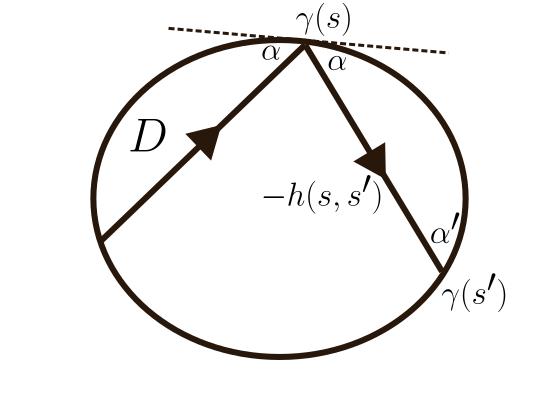
\includegraphics[width = 0.4\textwidth]{billiard2.png}
        \caption{ビリヤード系}
    \end{figure}

    この写像$T: (s, \alpha) \mapsto (s', \alpha')$を\textbf{ビリヤード写像}という.
    なお, $\gamma$の一周の長さを$L$としておくと, 
    この写像の定義域・値域(\textbf{相空間}という)は$(\mathbb{R}/L \mathbb{Z}) \times [0, \pi]$と書ける.
    (入射角$\alpha$が$0$や$\pi$の場合は, ビリヤードの運動によってその場を動かない(写像$T$の不動点)と考える.)

    さて, 実はこのビリヤード写像$T$は, 相空間$(\mathbb{R}/L \mathbb{Z}) \times [0, \pi]$上で
    次の$2$次微分形式($2$ - form)を保存することが知られている.

    \begin{theorem} \label{th:area}
        ビリヤード写像$T: (s, \alpha) \mapsto (s', \alpha')$は
        面積形式$\sin{\alpha} d s \wedge d \alpha$を保存する. 
        つまり, 
        \[
            \sin{\alpha} d s \wedge d \alpha = \sin{\alpha'} d s' \wedge d \alpha'.
        \]
    \end{theorem}

    このTheorem\ref{th:area}より, ビリヤード写像$T$は\textbf{面積保存写像}であるという.
    (ここで言う「面積」は, あくまで台$D$のいる平面での面積ではなく,
    相空間$(\mathbb{R}/L \mathbb{Z}) \times [0, \pi]$における面積のことである.)

    以下, この証明をやります.
\section{初等幾何的方法}
    こちらはよく知られている方法で, Birkhoffの証明を多少現代的に書いたもの.
    ビリヤード写像に触れている文献には大体書いているが,
    たとえば Tabachnikovの"Geometry and Billiards"や日本語のものだと柴山先生の『重点解説 ハミルトン系』などに載っている.

    \begin{proof}[Theorem \ref{th:area}の証明1]
        いま, $\gamma(s)$と$\gamma(s')$の距離(の$-1$倍)を$h(s, s')$と置く.
        $s$は弧長パラメータなので, 
        その微分$\pdv{\gamma(s)}{s}$は点$\gamma(s)$における単位接ベクトルである.
        内積を$\langle \cdot, \cdot \rangle$で表すことにすれば,
		\begin{align*}
			2 h(s, s') \pdv{h}{s'} &= \pdv{h^2}{s'}\\
            &= - \pdv{|\gamma(s) - \gamma(s')|^2}{s'}\\
            &= 2 \pdv{\langle \gamma(s) , \gamma(s') \rangle}{s'} - \pdv{\langle \gamma(s') , \gamma(s') \rangle}{s'} \\
			&= 2 \langle \gamma(s) , \pdv{\gamma(s')}{s'} \rangle - 2 \langle \gamma(s') , \pdv{\gamma(s')}{s'} \rangle \\
            &= 2\langle \gamma(s') - \gamma(x) , \pdv{\gamma(s')}{s'} \rangle \\
			&= - 2h(s, s') \cos \alpha'. \\
            \therefore \pdv{h}{s'} &= - \cos \alpha'.
        \end{align*}
        となる.
		同様にして, $\pdv{h}{s} = \cos \alpha$もわかる. 
        以上から, $\dd h = \cos \alpha \dd s - \cos \alpha' \dd s'$, 
        つまり 
        \[
            0 = \dd^2 h = \sin \alpha \dd s \land \dd \alpha - \sin \alpha' \dd s' \land \dd \alpha'
        \]
        となり,
        これから面積保存性$\sin \alpha \dd s \land \dd \alpha = \sin \alpha' \dd s' \land \dd \alpha'$がわかる.
    \end{proof}
    \section{その2: }


\section{その3: Poincar\'{e}-Cartan の積分不変式を用いた方法}

    以下は, ほとんどArnoldとAvezの"Ergodic Problems of Classical Mechanics"\cite{ArnoldAvez}のAPPENDIX 31に載っている内容です. 
    
    大まかに説明すると, 「ビリヤード写像を自由運動を記述するハミルトン系に適当なPoincar\'{e}断面を取ったときのPoincar\'{e}写像とみなしたとき, 
    Poincar\'{e}-Cartan の積分不変式から導かれる微分形式がなんと$\sin{\alpha} d s \wedge d \alpha$になっている」ということです.
    
    \subsection{ハミルトン系の準備: Poincar\'{e}-Cartan の積分不変式}
    まず準備としてハミルトン系とPoincar\'{e}-Cartan の積分不変式について解説します.
    このあたりはArnoldの"Mathematical Methods of Classical Mechanics"や
    Arnold, Kozlov, Neishtadtの"Mathematical Aspects of Classical and Celestial Mechanics"を大いに参考にしました.
    とはいえ, 多少は微分幾何に慣れてないとチンプンカンプンかもしれない(僕も微分幾何に弱いですが...)になってしまっていると思います. 

    Poincar\'{e}-Cartan の積分不変式のもっと直接的な導出が知りたい人は, 
    伊藤先生の『常微分方程式と解析力学』をオススメします.

    \vspace{\baselineskip}

    普通\textbf{ハミルトン系}というと, 
    $\mathbb{R}^{2n}$上の運動方程式で, ある関数(\textbf{ハミルトニアン})$H(p, q)$に対し, 
    \begin{equation} \label{ham}
        \dot{q}_{k} = \frac{\partial H}{\partial p_k}, \ \dot{p}_{k} = \frac{\partial H}{\partial q_k} \quad (k = 1, \cdots, n)
    \end{equation}
    と表されるものを指す.
    この解$(p(t), q(t))$上で$H$は$t$に依らず一定になる. 
    (多くの場合, $H$を力学的エネルギーの和(運動エネルギー + ポテンシャル)と解釈しても大丈夫.)

    ただ, 今回はPoincar\'{e}-Cartan の積分不変式を導きたい + 自分の勉強も兼ねて,
    少し特殊なやり方でハミルトン系を定めよう.
    \vspace{\baselineskip}
    $2n + 1$次元多様体$M^{2n + 1}$に, 適当な座標$(p, q, t) = (p_1, \cdots, p_n, q_1, \cdots, q_n, t)$を取る.
    $M^{2n + 1}$上の関数$H(p, q, t)$に対し, 
    次のような$1$次微分形式($1$-form)
    \begin{equation} \label{PC}
        \theta = p dq - H dt 
    \end{equation}
    を考える. 

    この1-form $\theta$により, ハミルトン系は次のようなやり方で決定される.

    その外微分$\omega = d \theta$は$2$-formであるが, 
    各点$x \in M^{2n + 1}$について, ある接ベクトル$\xi_x \neq 0$が存在し,
    \[
        \omega(\xi_x, \eta_x) = 0 \quad \forall \eta_x \in T_x M
    \]
    が存在する.
    なぜなら, $\omega$を表現する$(2n + 1)$次の歪対称行列を$A$とすれば, 
    \[
        \omega(\xi_x, \eta_x) = (A \xi_x, \eta_x)
    \]
    である. $A$は歪対称なので転置を取ると$A^{\textsf{T}} = -A$であるが,
    一方で$2n + 1$次なので, 
    \[
        \det(A) = \det(A^{\textsf{T}}) = \det(-A) = (-1)^{2n + 1} \det(A) = (-1) \det(A)
    \]
    となる. 結局, $\det(A) = 0$となり, $A$は非正則行列になるので, 
    同次方程式$A \xi_x = 0$が解を持つのである.

    この$A \xi_x = 0$を満たす$\xi_x$全体は線形空間をなすが, この次元が$1$しかないとき, 
    この$\xi_x$(を適当に正規化したもの)を$\omega$の\textbf{渦の方向}あるいは\textbf{特性方向}といい,
    渦の方向により定まるベクトル場$\xi = \{\xi_x\}$の積分曲線を$\omega$の\textbf{渦線}あるいは\textbf{特性曲線}という.
    $M$の中の閉曲線$\gamma_0$に対し, この曲線上の点から始めた渦線によって出来上がる曲面を$\omega$の\textbf{渦管}という.

    渦管の上で2-form$\omega$はどうなるかを確認しておこう.

    パラメータ$u$が入った$M^{2n + 1}$内の閉曲線$\gamma_0$を考える. ($\gamma_0(0) = \gamma_0(1)$とする.)
    この曲線上の各点$\gamma_0(u)$から出発する渦線を$x(s, u) = x^{s}(\gamma_0(u))$とすれば,
    閉曲線$\gamma_0$に対して定まる$\omega$の渦管$\Gamma$は
    $\Gamma = \{x(s, u) = x^{s}(\gamma_0(u))| s \in \mathbb{R}, u \in [0,1]\}$
    と書ける.

    $\Gamma$は$x: \mathbb{R} \times [0, 1] \ni (s, u) \rightarrow x^{s}(\gamma_0(u)) \in \Gamma$により
    座標$(s, u)$が入る.
    恒等写像$i: \Gamma \rightarrow M^{2n + 1}$により$\Gamma$を$M^{2n + 1}$に埋め込むと,
    $x(s, u) = (p(s, u) q(s, u) t(s, u))$と書いて, $p_s = \nabla_s p, p_u = \nabla_u p$などと表せば,
    \begin{align}
        i^{*} dp &= d p(s, u) = p_s ds + p_u du, \\ 
        i^{*} dq &= d q(s, u) = p_q ds + q_u du, \\
        i^{*} dt &= d t(s, u) = t_s ds + t_u du.
    \end{align}
    である.
    $M^{2n + 1}$上の$2$-form $\omega$の$\Gamma$への引き戻し$i^{*} \omega$を基底$ds, du$で表示すれば,
    \begin{align}
        i^{*} \omega 
        = [dp(s, u) \ dq(s, u) \ dt(s, u)] A
        \begin{bmatrix}
            dp(s, u)\\
            dq(s, u)\\
            dt(s, u)
        \end{bmatrix} 
        = [ds \ du] 
        \begin{bmatrix}
            p_s &q_s &t_s\\
            p_u &q_u &t_u
        \end{bmatrix}
        A
        \begin{bmatrix}
            p_s &p_u \\
            q_s &q_u \\
            t_s &t_u
        \end{bmatrix}
        \begin{bmatrix}
            ds\\
            du
        \end{bmatrix}
    \end{align}
    一方で, $x(s, u)$は渦の方向$\xi$の積分曲線なので, 
    $x_s = [p_s, q_s, t_s]^{\mathsf{T}}$は$A x_s = 0$を満たす.
    よって, 
    \[
        i^{*} \omega = [ds \ du] 
        \begin{bmatrix}
            x_s\\
            x_u
        \end{bmatrix}
        A
        \begin{bmatrix}
            x_s &x_u 
        \end{bmatrix}
        \begin{bmatrix}
            ds\\
            du
        \end{bmatrix}
        = [ds \ du]
        \begin{bmatrix}
            x_s^{\mathsf{T}} A x_s &x_s^{\mathsf{T}} A x_u \\
            x_u^{\mathsf{T}} A x_s &x_u^{\mathsf{T}} A x_u
        \end{bmatrix}
        \begin{bmatrix}
            ds\\
            du
        \end{bmatrix}
        = [ds \ du]
        \begin{bmatrix}
            0 &0 \\
            0 &x_u^{\mathsf{T}} A x_u
        \end{bmatrix}
        \begin{bmatrix}
            ds\\
            du
        \end{bmatrix}
    \]
    ここで, $A$が歪対称で$x_u^{\mathsf{T}} A x_u = (x_u^{\mathsf{T}} A x_u)^{\mathsf{T}} = - x_u^{\mathsf{T}} A x_u$であるから,
    $x_u^{\mathsf{T}} A x_u = 0$である.
    よって, 
    \[
        i^{*} \omega = 0
    \]
    となる.
    つまり, 渦管$\Gamma$の上では微分形式$\omega$は消失するのである.

    さて, この渦管の上での周回積分について, 次が成り立つ. 
    \begin{theorem} \label{Kl}
        $\omega = d \theta$の渦管$\Gamma$上の, 
        (渦管を一周する)同じ向きの閉曲線$\gamma_0, \gamma_1$を考えると,
        渦線が$\gamma_0$から$\gamma_1$に向けて伸びているとすれば,
        \begin{equation} \label{uzu}
            \int_{\gamma_0} \theta = \int_{\gamma_1} \theta.
        \end{equation}
    \end{theorem}

    この定理は, 渦の方向により定まるベクトル場の運動について, 
    \begin{equation} \label{inv}
        I(s) = \int_{x^{s}(\gamma_0)} \theta
    \end{equation}
    が$s$に依らず不変であることを示唆している(\textbf{ケルビンの渦定理}の一般化).

    \begin{proof}
        Stokesの定理から,
        \[
            \int_{\Gamma} \omega = \int_{\Gamma} d \theta = \int_{\gamma_0} \theta -\int_{\gamma_1} \theta
        \]
        であるが, 渦管の上で$\omega$は消失するので, 左辺は$0$である.
        よって, 
        \begin{equation}
            \int_{\gamma_0} \theta - \int_{\gamma_1} \theta = 0
        \end{equation}
        となり, 題意が示される.
        % 初期点$x_0 \in \gamma_0$を出発した渦線を$x(s, x_0)$と書き, 
        % 各$s \in [0, 1]$に対して写像$x^{s}: \gamma_0 \ni x_0 \mapsto x^{s}(x_0) = x(s, x_0) \in x^{s}(\gamma_0)$を考えて,
        % \[
        %     I(t) = \int_{x^{t}(\gamma_0)} \theta
        % \]
        % とする.
        
        % まず, $x^{0} = \mathrm{id}$(恒等写像)であるから
        % \[
        %     I(0) = \int_{\gamma_0} \theta
        % \]
        % である.

        % 次に, 任意の時刻$s = \tau$を固定し,
        % \[
        %     \left.\frac{d}{d s} I(s) \right|_{s = \tau} 
        %     = \left. \frac{d}{d s}\right|_{s = \tau} \int_{x(s, \gamma_0)} \theta 
        % \]
        % を考える.
        % \begin{align}
        %     \left.\frac{d}{d s}\right|_{s = \tau} \int_{x(s, \gamma_0)} \theta 
        %     &= \lim_{s \rightarrow 0} \frac{1}{s} \qty{\int_{x(s + \tau, \gamma_0)} \theta - \int_{x(\tau, \gamma_0)} \theta } \\
        %     &= \lim_{s \rightarrow 0} \frac{1}{s} \qty{\int_{\gamma_0} (x^{s + \tau})^{*} \theta - \int_{\gamma_0} (x^{\tau})^{*} \theta } \\
        %     &= \lim_{s \rightarrow 0} \frac{1}{s} \qty{\int_{\gamma_0} (x^{s})^{*} \theta - \theta } \\
        %     &=  \int_{\gamma_0} \lim_{s \rightarrow 0} (x^{\tau})^{*} \frac{1}{s} ((x^{s})^{*} \theta - \theta).
        % \end{align}
        % さて, 渦線の定義から$x^{s}$は渦の方向により定まるベクトル場$\xi = \{\xi_x\}$のフローである.
        % そのため, ベクトル場$\xi$によるLie微分を$L_{\xi}$と書けば, 
        % \[
        %     \lim_{s \rightarrow 0} \frac{1}{s}((x^{s})^{*} \theta - \theta) = L_{\xi} \theta.
        % \]
        % しかし, Cartanの公式$L_{\xi} = \iota(\xi) d \theta + d \iota(\xi) \theta$と 
        % $\xi_x$は$\omega$の渦の方向だから$\iota(\xi) d \theta= \omega(\xi, \cdot) = 0$
        % であることを用いると, 
        % \[
        %     (x^{\tau})^{*} L_{\xi} \theta = (x^{\tau})^{*} d \iota(\xi) \theta =  d (x^{\tau})^{*} \iota(\xi) \theta.
        % \]
        % 結局, 
        % \[
        %     \left.\frac{d}{d s}\right|_{s = \tau} \int_{x(s, \gamma_0)} \theta = \int_{\gamma_0} L_{\xi} \theta = \int_{\gamma_0} d (x^{\tau})^{*} \iota(\xi) \theta
        % \]
        % しかし, Stokesの定理から
        % \[
        %     \int_{\gamma_0} d \iota(\xi) \theta = \int_{\partial \gamma_0} (x^{\tau})^{*} \iota(\xi) \theta = 0. \quad (\therefore \partial \gamma_0 = \varnothing).
        % \]
        % 以上から, 
        % \[
        %     \left.\frac{d}{d s} I(s) \right|_{s = \tau} = 0
        % \]
        % である. $\tau$は任意に選べたから, 
        % \[
        %     I(\tau) = I(0) = \int_{\gamma_0} \theta
        % \]
        % 特に, $\tau = 1$と置けば, 式\eqref{uzu}が得られる.
    \end{proof}
    
    ところで, $1$-form $\theta$は式\eqref{PC}で具体的に与えていた. 
    このときの$\omega = d \theta$に対する積分曲線(渦線)はなんであろうか?

    具体的に$\omega$の表現行列$A$を計算しよう. $p = (p_1, \cdots, p_n), q =(q_1, \cdots, q_n)$として,
    $H_p = \nabla_{p} H(p, q, t), H_q = \nabla_{Q} H(p, q, t)$で表せば, 
    \[
        A = 
        \begin{bmatrix}
            O_n & E_n & - H_p \\
            - E_n & O_n & - H_q \\
            H_p^{\mathsf{T}} & H_q^{\mathsf{T}} & 0
        \end{bmatrix}
    \]
    となる. ただし, $E_n$は$n$次の単位行列, $O_n$は$n$次の零行列である.

    この表現行列$A$の右上の$2n$次正方行列は正則であるため, 
    同次方程式$AX = 0$の解空間は$1$次元であり, 上の話が適用できる.
    解空間の元$X \in TM$は
    \[
        X = \sum_{k} X_k \frac{\partial}{\partial p_k} + X_{k+n} \frac{\partial}{\partial q_k} + X_t \frac{\partial}{\partial t}
    \] 
    と書けるが, 特に$X_t \neq 0$である.\\
    (なぜなら, $AX = 0$より
    \[  AX = 
        \begin{bmatrix}
            X_{k+n}  -H_p X_t \\
            -X_k -H_q X_t\\
            H_p X_k + H_q X_{k+n}
        \end{bmatrix} = 0
    \]
    であるので, もし$X_t = 0$なら$X_k = X_{k+n} = X_t = 0$となり, $X = 0$になってしまう.)
    
    そのため, 特に$X_t = 1$となるものを渦の方向として定めても良い. このとき, $AX = 0$から他の成分は
    \[
        X_k = - H_{q_k}, \ X_{k+n} = H_{p_k} \quad (k = 1, \cdots n)
    \]
    と決定する.
    したがって, 渦の方向の定めるベクトル場$X$は
    \[
        X = \sum_{k} - H_{q_k} \frac{\partial}{\partial p_k} +  H_{p_k} \frac{\partial}{\partial q_k} + \frac{\partial}{\partial t}
    \]
    であり, この積分曲線$x(s, x_0) = (p(s, x_0), q(s, x_0) t(s, x_0))$の満たすべき方程式は拡張したハミルトン系
    \begin{equation} \label{etd}
        \dot{q}_k = \frac{\partial H}{\partial p_k}, \ \dot{p}_k = -\frac{\partial H}{\partial q_k},\  \dot{t} = 1 \quad (k = 1, \cdots, n)
    \end{equation}
    にほかならない. 
    Theorem\ref{Kl}から, 拡張したハミルトン系\eqref{etd}のフロー$x^s$に沿って, 積分
    \begin{equation} \label{PC-inv}
        \int_{x^{s}(\gamma_0)} p dq - H dt
    \end{equation}
    の値は不変である. 
    \begin{theorem} \label{PC-etd}
        拡張したハミルトン系\eqref{etd}について, 
        相空間内の閉曲線$\gamma_0$と, フロー$x^{s}$により描かれる管$\gamma_1 = x^{1}(\gamma_0)$について,
        \begin{equation} \label{eq:PC-inv}
            \int_{\gamma_0} p dq - H dt = \int_{\gamma_1} p dq - H dt.
        \end{equation}
    \end{theorem}
    ハミルトン系\eqref{ham}は\eqref{etd}の解を$(p, q)$平面に射影したものに過ぎないが, 
    上の定理をハミルトンフロー$\phi^{t}$により$\gamma_1 = \phi^{t}(\gamma_0)$にすれば, 
    $\gamma_0, \gamma_1$上で$t$は定数であり$dt = 0$となるので, 次が成立する;
    \begin{theorem} \label{PC-ham}
        ハミルトン系\eqref{ham}について, 
        相空間内の閉曲線$\gamma_0$と, ハミルトンフロー$\phi^{t}$により描かれる管$\phi^{t}(\gamma_0)$について,
        \begin{equation} \label{eq:P-inv}
            \int_{\gamma_0} p dq = \int_{\gamma_1} p dq.
        \end{equation}
    \end{theorem}
    
    以上から, ハミルトン系\eqref{ham}は式\eqref{PC}で決まる1-form$\theta$から導出できる.
    また, その拡張したハミルトン系\eqref{etd}には, 積分で書ける不変量\eqref{PC-inv}を持つ.
    この不変量\eqref{PC-inv}を\textbf{Poincar\'{e}-Cartan の積分不変式}という.

    \subsection{ハミルトン系のPoincar\'{e} 写像}

    $n$自由度ハミルトン系\eqref{ham}に話を戻す.
    この系の相空間は$2n$次元の多様体になるが, その断面$\Sigma$を$H = h, q_1 = 0$で与えると, 
    $\Sigma$は等エネルギー$H = h$を持つ$2n - 2$次元部分多様体をなす.

    ある領域$\Sigma_0 \subset \Sigma$で局所座標$(P, Q) = (p_2, \cdots, p_n, q_2, \cdots, q_n)$が取れたとし,
    かつこの領域で上の方程式について$\dot{q}_1 \neq 0$が成り立っているとき, 
    断面$\Sigma$をsurface of section とか Poincar\'{e} sectionとか言う.
    (日本だと多分「Poincar\'{e} 断面」と呼ぶケースが多いと思う.)

    いま, 点$x \in \Sigma_0$であって, 
    初期点$x$についてのハミルトン系の解がしばらくして$\Sigma_0$に戻って来るようなものを考える.
    このとき, $\dot{q}_1 \neq 0$より, $x$に十分近い点$x' \in \Sigma_0$を通過する解は
    またいずれ$\Sigma_0$に戻って来て, $\Sigma_0$を横断する.
    この$x'$の定義できるような$x$の近傍$\Sigma_1 \subset \Sigma_0 \subset \Sigma$について, 
    $\Sigma_0$内の再帰した点を$Ax'$とすれば, 
    写像$A: \Sigma_1 \rightarrow \Sigma_0$が定義できる. 
    (このような写像を\textbf{Poincar\'{e}写像}という.)

    \begin{theorem} \label{th:A31.5}
        上で定めたハミルトン系のPoincar\'{e}写像$A: \Sigma_1 \rightarrow \Sigma_0$は正準的である.
        すなわち, $\Sigma_1$内の任意の閉曲線$\gamma$について, 
        \begin{equation} \label{A31.5}
            \int_{\gamma} P dQ = \int_{A \gamma} P dQ.
        \end{equation}
        である.
        ただし, $P dQ = \sum_{k = 2}^{n} p_k d q_k$.
    \end{theorem}

    \begin{proof}
        拡張したハミルトン系\eqref{etd}の下で考え, 
        拡張した相空間$\{(p, q, t)\}$上での閉曲線をそれぞれ$\gamma', A\gamma'$とする.
        ($\gamma'$は$t = 0$の面の上での$\gamma_0$にほかならないが, 
        再帰時間は点ごとに異なるため$A \gamma'$の各点での$t$座標は一致しない)

        Poincar\'{e}-Cartanの積分不変式(Theorem\ref{PC-etd})より
        \begin{equation}
            \int_{\gamma'} p dq - H dt = \int_{A \gamma'} p dq - H dt.
        \end{equation}
        となる.
        ここで, $\gamma$および$A\gamma$は等エネルギー面(つまり, $H = $定数である面)の上にあるので,
        \begin{equation}
            \int_{\gamma'} H dt = \int_{A \gamma'} H dt.
        \end{equation}
        また, $\gamma'$上は$t = 0$で一定なので,$dt = 0$であり,
        \begin{equation}
            \int_{\gamma'} H dt = 0.
        \end{equation}
        したがって, 
        \[
            \int_{\gamma'} p dq = \int_{\gamma} p dq, \ \int_{A \gamma'} p dq = \int_{A \gamma} p dq
        \]
        $q_1$は$\Sigma_1 \subset \Sigma$上で一定なので, $\gamma', A \gamma'$上で$dq = 0$であり, 
        \[
            \int_{\gamma'} p_1 dq_1 = \int_{A \gamma'} p dq = 0.
        \]
        したがって,
        \[
            \int_{\gamma} P dQ = \int_{\gamma'} p dq - H dt = \int_{A \gamma'} p dq - H dt = \int_{A \gamma} P dQ.
        \]
        となり,\eqref{A31.5}が示された.

    \end{proof}

    \subsection{ビリヤード系への応用}
        \begin{proof}[Theorem\ref{th:area}の証明その3]
            いま, 台$D \subset \mathbb{R}^2$内を自由運動(等速直線運動)するボールを考える.
            この質点の位置と速度をまとめて$(x, v) = (x_1, x_2, v_1, v_2)$と置くと, 運動方程式は
            \[
                \dot{x}_i = v_{i}, \ \dot{v}_i = 0 \quad (i = 1, 2)
            \]  
            である. この運動のハミルトニアン$H(x, v)$は運動エネルギーだけ, つまり
            \[
                H(x, v) = \frac{1}{2} (v_1^2 + v_2^2).
            \]
            となる.

            ここで, 原点$O$が台の境界$\gamma = \partial D$の上になるようにし, 
            $(q_1, q_2)$を, 
            $q_1$をボールの位置$M$から最も近い境界上の点$N$までの距離,
            $q_2$を原点$O$から点$N$までの弧の長さ
            と定める.
            $q = (q_1, q_2)$は$D$全体では定義できないが,
            $\gamma = (\gamma_1, \gamma_2)$の近傍に限って言えば正しく定まる.

            \begin{figure}[h]
                \centering
                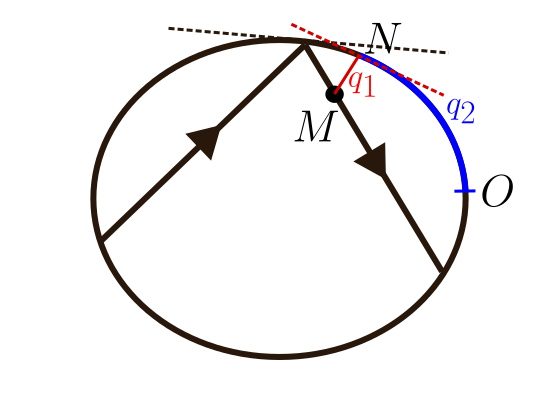
\includegraphics[width = 0.4\textwidth]{billiard_Hamilton.png}
                \caption{ハミルトン系(自由運動)としてのビリヤード}
            \end{figure}

            境界上の各点$\gamma(s)$における接ベクトルを$\vec{t}(s)$,
            法ベクトルを$\vec{n}(s)$と書けば,
            $\vec{t}(s)$は$\gamma(s)$の弧長パラメータでの微分であり,
            $\vec{n}(s)$は$\vec{t}(s)$を$\pi/2$だけ反時計回りに回転させたものなので,
            \[
                \vec{t}(s) = (\gamma'_1(s), \gamma'_2(s)), \ \vec{n}(s) = (- \gamma'_2(s), \gamma'_1(s))
            \]
            となる.
            $\vec{ON} = (\gamma_1(q_2), \gamma_2(q_2))$であり,
            $\vec{NM} = q_1 \vec{n}(q_2)$なので,
            $x = (x_1, x_2)$から$q = (q_1, q_2)$の点変換は
            \[
                x_1 = \gamma_1(q_2) - q_1 \gamma'_2(q_2), \ x_2 = \gamma_2(q_2) + q_1 \gamma'_1(q_2)
            \]  
            と書ける. (ここのプライムは$s$での微分.)

            $\gamma$の近傍(とその上での定まる速度ベクトル全体)のなす相空間内の開集合に対し,
            点変換$q \mapsto x = x(q_1, q_2)$から定まる$(x, v)$から$(q, p) = $への正準変換を考えることができる.
            具体的には, 正準変換の母関数$S(v, q)$を
            \[
                S(v, q) = v_1 x_1(q_1, q_2) + v_2 x_2(q_1, q_2) = v_1(\gamma_1(q_2) - q_1 \gamma'_2(q_2)) + v_2 (\gamma_2(q_2) + q_1 \gamma'_1(q_2))
            \]
            とすれば, 点変換に対応する正準変換が定まり, このとき曲率を$\kappa$で書けば, 
            運動量$p = (p_1, p_2)$は
            \begin{align}
                p_1 &= \frac{\partial S}{\partial q_1} = - v_1 \gamma'_2(q_2) + v_2 \gamma'_1(q_2) \\
                &= v \cdot \vec{n}(q_2), \\
                p_2 &= \frac{\partial S}{\partial q_2} = v_1 (\gamma'_1(q_2) - q_1 \gamma''_2(q_2)) + v_2 (\gamma'_2(q_2) - q_1 \gamma''_1(q_2)), \\
                &= v \cdot \vec{t}(q_2) + q_1 \kappa(q_2) v \cdot \vec{n}(q_2).
            \end{align}
            で表示できる.

            さて, このハミルトン系に対し, $H = 1/2, q_1 = 0$でのPoincar\'{e}断面$\Sigma$を取る.
            これは, $|v| = 1$かつボールが$\gamma$上(つまり, 壁にぶつかる瞬間)という条件にほかならず,
            ビリヤード写像$T$はこのPoincar\'{e}断面$\Sigma$についてのPoincar\'{e}写像とみることができる.
            すなわち, Theorem\ref{th:A31.5}から$T$は$\Sigma_1$上で$2$-form $d p_2 \wedge d q_2$を保存する.

            運動量$p$の式に$|v| = 1, q_1 = 0$を入れてみると, 入射角$\alpha$に対して
            \begin{align}
                p_1 &= v \cdot \vec{n}(q_2) = \sin{\alpha}, \\
                p_2 &= v \cdot \vec{t}(q_2) = \cos{\alpha}
            \end{align}
            であるから, $\Sigma_0$上で$d p_2 \wedge d q_2 = d (\cos{\alpha}) \wedge d q_2 = \sin{\alpha} d q_2 \wedge d \alpha$.
            $q_2$は$\gamma$の弧長パラメータだったから, これは$\sin{\alpha} d s \wedge d \alpha$にほかならない.
        \end{proof}



        
    

    \begin{thebibliography}{10}
    \nocite{*}
	\bibitem{ArnoldAvez} V.I.Arnold, A.Avez. Ergodic Problems of Classical Mechanics, Benjamin, (1968)
\end{thebibliography}
\end{document}